\documentclass{article}
\usepackage{xeCJK}
\usepackage{makeidx}
\usepackage{hyperref}
\usepackage{amsmath}
\usepackage{xcolor}
\usepackage{graphicx}

\title{Machine Learning Notes}
\author{Haotian Chen}
\date{}

\makeatletter
\renewcommand\paragraph{\@startsection{paragraph}{4}{\z@}%
                                     {-3.25ex\@plus -1ex \@minus -.2ex}%
                                     {1.5ex \@plus .2ex}%
                                     {\normalfont\normalsize\bfseries}}
\makeatletter

\hypersetup{
    colorlinks=true,
    linkcolor=blue,
    urlcolor=cyan,
}

\setcounter{tocdepth}{4}
\setcounter{secnumdepth}{4}

\makeindex



\begin{document}

\maketitle

\clearpage

\tableofcontents{}

\clearpage

\section{Machine Learning Introduction}

A computer program is said to learn
from experience E with respect to some task T
and some performance measure P, if its
performance on T, as measured by P, improves
with experience E. 

\subsection{Supervised Learning}

Supervised learning algorithms build a mathematical model 
of a set of data that contains both the inputs and the desired 
outputs.

\bigskip

\noindent In supervised learning, each example is a 
pair consisting of an input object (typically a vector) 
and a desired output value (also called the supervisory signal).

\subsubsection{Regression}

Regression analysis is a set of statistical processes 
for estimating the relationships between a dependent 
variable (often called the `outcome variable') and one 
or more independent variables (often called `predictors', 
`covariates', or `features').

\bigskip

\noindent \textbf{Training(Learning) Process:}

\noindent \textit{observed data(training set)} $\rightarrow$ \textit{learning algorithm} $\rightarrow$ \textit{h(hypothesis)}

\noindent \textit{hypothesis:} 假设

\bigskip

\noindent \textbf{Predicting Process:}

\noindent \textit{independent variable} $\rightarrow$ \textit{h(hypothesis)} $\rightarrow$ \textit{dependent variable}

\subsubsection{Classification}

Classification is the problem of identifying to which 
of a set of categories (sub-populations) a new observation 
belongs, on the basis of a training set of data containing 
observations (or instances) whose category membership is known.

\subsection{Unsupervised Learning}

Unsupervised learning algorithms take a set of data that 
contains only inputs, and find structure in the data, like 
grouping or clustering of data points.

\bigskip

\noindent Draw inferences from data sets consisting of input 
data without labeled responses.

\subsection{Reinforcement learning}
       
Reinforcement learning is an area of machine learning concerned 
with how software agents ought to take actions in an environment 
so as to maximize some notion of cumulative reward.

\section{Regression}

\subsection{Linear Regression(from \href{https://en.wikipedia.org/wiki/Linear_regression\#:~:text=In\%20statistics\%2C\%20linear\%20regression\%20is,is\%20called\%20simple\%20linear\%20regression.}{Wikipedia})}

Given a data set \(\{y_i, x_{i1}, ..., x_{ip}\}_{i=1}^n\) of n statistical units, a linear regression model assumes that the relationship between the dependent variable y and the p-vector of regressors x is linear.

\[y_i = \beta_0 + \beta_{1}x_{i1} + \dots + \beta_{p}x_{ip} + \epsilon_i, \: i = 1, \dots, n\]
\[y = X\beta + \epsilon\]

\noindent where

\bigskip

\(
y = 
\begin{bmatrix}
y_1\\
y_2\\
\vdots\\
y_n
\end{bmatrix}
,
X = 
\begin{bmatrix}
x_1^T\\
x_2^T\\
\vdots\\
x_n^T
\end{bmatrix} = 
\begin{bmatrix}
1 & x_{11} & \dots & x_{1p}\\
1 & x_{21} & \dots & x_{2p}\\
\vdots & \vdots & \ddots & \vdots\\
1 & x_{n1} & \dots & x_{np}
\end{bmatrix}
,
\beta = 
\begin{bmatrix}
\beta_0\\
\beta_1\\
\vdots\\
\beta_p
\end{bmatrix}
,
\epsilon = 
\begin{bmatrix}
\epsilon_1\\
\epsilon_2\\
\vdots\\
\epsilon_n
\end{bmatrix}
\)

\bigskip

\noindent \(y\) is a vector of observed values \(y_{i}\ (i=1,\ldots ,n)\) of the variable called the regressand, endogenous variable, response variable, measured variable, criterion variable, or dependent variable.

\bigskip

\noindent \(X\) may be seen as a matrix of row-vectors \(x_{i}\) or of n-dimensional column-vectors \(X_{j}\), which are known as regressors, exogenous variables, explanatory variables, covariates, input variables, predictor variables, or independent variables. Usually a constant is included as one of the regressors. In particular, \(x_{i0} = 1\) for \(i = 1, \dots, n\). The corresponding element of \(\beta\) is called the intercept. 

\bigskip

\noindent \(\beta\) is a \((p + 1)\)-dimensional parameter vector, where \(\beta_{0}\) is the intercept term (if one is included in the model—otherwise \(\beta\) is p-dimensional). Its elements are known as effects or regression coefficients (although the latter term is sometimes reserved for the estimated effects).

\bigskip

\noindent \(\epsilon\) is a vector of values \(\epsilon_{i}\). This part of the model is called the error term, disturbance term, or sometimes noise (in contrast with the ``signal" provided by the rest of the model).

\bigskip

\noindent \textbf{Matrix Concepts}

\bigskip

\noindent \textbf{identity matrix} \(I\)(or \(I_{n \times n}\)):

\[A \cdot I = I \cdot A = A\]

\[
I = 
\begin{bmatrix}
1 & 0 & \dots & 0 & 0\\
0 & 1 & \dots & 0 & 0\\
\vdots & \vdots & \ddots & \vdots & \vdots\\
0 & 0 & \dots & 1 & 0\\
0 & 0 & \dots & 0 & 1
\end{bmatrix}
\]

\noindent \textbf{inverse matrix} \(A^{-1}\): If \(A\) is an \(m \times m\) matrix, and if it has an inverse.
\[A \cdot A^{-1} = A^{-1} \cdot A = I\]

\noindent \textbf{transpose matrix} \(A^{T}\): Let \(A\) be an \(m \times n\) matrix. Then \(A^T\) is an \(n \times m\) matrix.
\[A^T_{ij} = A_{ji}\]

\subsubsection{Linear Regression Learning (from \href{https://www.coursera.org/learn/machine-learning}{Machine Learning course})}

\noindent For convenience reasons, define \(x_0 = 1\)
\[
x = 
\begin{bmatrix}
x_0\\
x_1\\
\vdots\\
x_n
\end{bmatrix}
,
\theta = 
\begin{bmatrix}
\theta_0\\
\theta_1\\
\vdots\\
\theta_n
\end{bmatrix}
\]

\noindent \textbf{hypothesis}:
\[y = h_{\theta}(x) = \theta^T x = \theta_0 + \theta_1 x_1 + \theta_2 x_2 + \dots + \theta_n x_n\]

\noindent \textbf{training data}:
\[(x^{(i)}, y^{(i)})\:for\:i = 1, \dots, m\]

\noindent \textbf{cost function}:
\[J(\theta) = \frac{1}{2m} \sum_{i = 1}^m (h_{\theta}(x^{(i)}) - y^{(i)})^2\]

\noindent goal:
\[\underset{\theta}{\text{minimize}} \: J(\theta)\]

\noindent \textbf{gradient descent}:

\noindent repeat until convergence \{
\[\theta_j =: \theta_j - \alpha \frac{\partial}{\partial \theta_j} J(\theta) = \theta_j - \alpha \frac{1}{m} \sum_{i = 1}^m (h_{\theta}(x^{(i)}) - y^{(i)}) x^{(i)}_j\]
\centerline{simultaneously update \(\theta_j\) for \(j = 0, \dots, n\)}
\}

\bigskip

\noindent \textbf{vectorized implementation}:

\noindent repeat until convergence \{
\[\theta =: \theta - \alpha \frac{1}{m} \sum_{i = 1}^m (h_{\theta}(x^{(i)}) - y^{(i)}) x^{(i)}\]
\}

\bigskip

\noindent \textbf{batch}:

\noindent Each step of gradient descent uses all the training examples.

\bigskip

\noindent \textbf{Feature scaling}:

\noindent The range of all features should be normalized so that each feature contributes approximately proportionately to the result. Also it helps gradient descent converge much faster.

\bigskip

\noindent \textbf{mean normalization}: (don't apply to \(x_0\))

\[x_i = \frac{x_i - mean(x_i)}{max(x_i) - min(x_i)}\]

\bigskip

\noindent \textbf{standardization}: (don't apply to \(x_0\)) \textcolor{orange}{ * math stuff needed for this part}

\noindent Feature standardization makes the values of each feature in the data have zero-mean (when subtracting the mean in the numerator) and unit-variance.

\[x_i = \frac{x_i - mean(x_i)}{std(x_i)}\]

\[std(x_i) = \sqrt{ \frac{1}{m} \sum_{j = 1}^m (x^{(j)}_i - mean(x_i))^2}\]

\noindent \textbf{learning rate} \(\alpha\):

\noindent If \(\alpha\) is too small: slow convergence.

\noindent If \(\alpha\) is too large: may not decrease on every iteration and thus may not converge.

\noindent try a range of learning rate to find a good one:

\[\alpha = \dots, 0.001, \dots, 0.01, \dots, 0.1, \dots\]

\noindent \textbf{Feature choosing}:

\noindent Choose the right features to fit the data set.

\noindent housing price example, choose from:

\[h_{\theta}(x) = \theta_0 + \theta_1 \times frontage + \theta_2 \times depth\]
\[h_{\theta}(x) = \theta_0 + \theta_1 \times area\]

\noindent \textbf{polynomial regression}:

\noindent Use the polynomial model with the machinery of multivariant linear regression.

\noindent housing price example, choose from:

\[h_{\theta}(x) = \theta_0 + \theta_1 \times area + \theta_2 \times area^2\]
\[h_{\theta}(x) = \theta_0 + \theta_1 \times area + \theta_2 \times \sqrt{area}\]

\subsubsection{Normal Equation}

\noindent Let:

\[
X = 
\begin{bmatrix}
(x^{(1)})^T\\
(x^{(2)})^T\\
\vdots\\
(x^{(m)})^T
\end{bmatrix}
,
y = 
\begin{bmatrix}
y^{(1)}\\
y^{(2)}\\
\vdots\\
y^{(m)}
\end{bmatrix}
\]

\noindent Calculate best \(\theta\): \textcolor{orange}{ * math stuff needed for this part}

\[
\theta = (X^TX)^{-1}X^Ty
\]

\noindent If \(X^TX\) is noninvertible, the common causes might be having:

\noindent 1. Redundant features, where two features are very closely related (i.e. they are linearly dependent)

\noindent 2. Too many features (e.g. \(m < n\)). In this case, delete some features or use "regularization".

\bigskip

\noindent \textbf{Gradient Descent} vs \textbf{Normal Equation}:

\begin{center}
\begin{tabular}{ | c | c | } 
\hline
\textbf{Gradient Descent} & \textbf{Normal Equation} \\ 
\hline
Need to choose \(\alpha\) & No need to choose \(\alpha\) \\ 
\hline
Needs many iterations & No need to iterate \\ 
\hline
\(O(kn^2)\) & \(O(n^3)\). Need to calculate \((X^TX)^{-1}\) \\ 
\hline
Works well when n is large & Slow if n is very large \\ 
\hline
\end{tabular}
\end{center}

\noindent \textbf{Vectorized Cost Function}: \textcolor{orange}{ * math stuff needed for this part}

\[J(\theta) = \frac{1}{2m} (X\theta - y)^T(X\theta - y)\]

\subsection{Logistic Regression}

\noindent \textbf{sigmoid function:} (Logistic Function)

\noindent Maps any real number from \((-\infty, +\infty)\) to the \((0, 1)\) interval.
\[g(z) = \frac{1}{1 + e^{-z}}\]

\noindent \textbf{hypothesis:}
\[
h_{\theta}(x) 
= g(\theta^T x)
= \frac{1}{1 + e^{-\theta^T x}}
\]

\noindent \(h_{\theta}(x)\) will give us the probability that our output is 1. Our probability that our prediction is 0 is just the complement of our probability that it is 1.

\[
h_{\theta} (x) 
= P(y = 1 | x ; \theta)
= 1 - P(y = 0 | x ; \theta)
\]
\[P(y = 1 | x ; \theta) + P(y = 0 | x ; \theta) = 1\]

\noindent \textbf{decision boundary:}

\noindent In order to get our discrete 0 or 1 classification, we can translate the output of the hypothesis function as follows:

\[h_{\theta} (x) \geq 0.5 \rightarrow y = 1\]
\[h_{\theta} (x) < 0.5 \rightarrow y = 0\]

\noindent Decision is made when:

\[g(\theta^T x) \geq 0.5, \text{ when } \theta^T x \geq 0\]
\[g(\theta^T x) < 0.5, \text{ when } \theta^T x < 0\]

\noindent Now we get:

\[\theta^T x \geq 0 \rightarrow y = 1\]
\[\theta^T x < 0 \rightarrow y = 0\]

\noindent The decision boundary is the line that separates the area where \(y = 0\) and where \(y = 1\):
\[\theta^T x = 0\]

\noindent \textbf{cost function:}

\noindent If we use the the same cost function that we use for linear regression for logistic regression, the cost function will have many local optima. It will not be a convex function. Instead, we construct logistic regression cost function as follows:

\[J(\theta) = \frac{1}{m} \sum_{i = 1}^m Cost(h_{\theta}(x^{(i)}), y^{(i)})\]
\[Cost(h_{\theta}(x), y) = -log(h_{\theta}(x)), \text{ if } y = 1\]
\[Cost(h_{\theta}(x), y) = -log(1 - h_{\theta}(x)), \text{ if } y = 0\]

\noindent We can find it guarantees that \(J(\theta)\) is convex for logistic regression: \textcolor{orange}{ * math stuff needed for this part}
\[
Cost(h_{\theta}(x), y) = 0 \text{ if }
h_{\theta}(x) = y, \text{ at } h_{\theta}(x) = y = 0 \text{ and } 
h_{\theta}(x) = y = 1
\]
\[
Cost(h_{\theta}(x), y) \rightarrow +\infty
\text{ if } y = 0 \text{ and }
h_{\theta}(x) \rightarrow 1
\]
\[
Cost(h_{\theta}(x), y) \rightarrow +\infty
\text{ if } y = 1 \text{ and }
h_{\theta}(x) \rightarrow 0
\]

\noindent We can compress our cost function's two conditional cases into one case:
\[Cost(h_{\theta} (x), y) 
= - y log(h_{\theta} (x)) - (1 - y) log(1 - h_{\theta} (x))\]

\noindent \textbf{simplified cost function:}
\[J(\theta) = - \frac{1}{m} \sum_{i = 1}^{m} [y^{(i)} log(h_{\theta} (x^{(i)})) + (1 - y^{(i)}) log(1 - h_{\theta} (x^{(i)}))]\]

\noindent \textbf{vectorized cost function:}
\[h = g(X\theta)\]
\[J(\theta) = \frac{1}{m} (- y^T log(h) - (1 - y)^T log(1 - h))\]

\noindent \textbf{gradient descent:}

\noindent repeat until convergence \{
\[\theta_j =: \theta_j - \alpha \frac{\partial}{\partial \theta_j} J(\theta) = \theta_j - \alpha \frac{1}{m} \sum_{i = 1}^m (h_{\theta}(x^{(i)}) - y^{(i)}) x^{(i)}_j\]
\centerline{simultaneously update \(\theta_j\) for \(j = 0, \dots, n\)}
\}

\bigskip

\noindent \textbf{vectorized implementation}:

\noindent repeat until convergence \{
\[\theta =: \theta - \alpha \frac{1}{m} X^T (g(X\theta) - y)\]
\}

\bigskip

\noindent \textbf{advanced optimization methods}:

\noindent With the same cost function, we can choose different optimization method to optimize \(\theta\): \textcolor{orange}{ * math stuff needed for this part}

\begin{itemize}
\item gradient descent
\item conjugate gradient
\item BFGS
\item L-BFGS
\item ...
\end{itemize}

\bigskip

\noindent \textbf{multiclass classification}:

\noindent Instead of \(y = \{0, 1\}\), we will expand our definition so that \(y = \{0, 1, ..., n\}\). Then we divide our problem into n+1 binary classification problems, by constructing n + 1 hypothesis functions; in each one, we choose one class and then lump all the others into a single second class, then predict the probability that \(y\) is a member of the chosen class.

\bigskip

\noindent To summarize: 

\noindent Train a logistic regression classifier \(h_{\theta}^{(i)}(x)\) for each class to predict the probability that \(y = i\). On a new input \(x\), to make a prediction, pick the class \(i\) that maximizes \(h_{\theta} ^{(i)}(x)\).

\[y \in \{0, 1 ... n\}\] 
\[h_{\theta}^{(0)}(x) = P(y = 0 | x ; \theta)\]
\[h_{\theta}^{(1)}(x) = P(y = 1 | x ; \theta)\]
\[\cdots\]
\[h_{\theta}^{(n)}(x) = P(y = n | x ; \theta)\] 
\[\text{prediction} = \max_i(h_{\theta}^{(i)}(x))\]

\subsection{Overfitting Problem}

\noindent \textbf{underfitting}:

\noindent High bias, which means hypothesis fits training data poorly, is usually caused by a function that is too simple or using too few features. 

\bigskip

\noindent \textbf{overfitting}:

\noindent High variance, which means hypothesis fits training data well, but does not generalize well to predict new data. It is usually caused by a complicated function with too many features.

\bigskip

\noindent \textbf{address overfitting}:

\begin{enumerate}
\item Reduce the number of features:
\begin{itemize}
\item Manually select which features to keep.
\item Use a model selection algorithm (studied later in the course).
\end{itemize}
\item Regularization:
\begin{itemize}
\item Keep all the features, but reduce the magnitude of parameters \(\theta_j\).
\item Regularization works well when we have a lot of slightly useful features.
\end{itemize}
\end{enumerate}

\subsubsection{Linear Regression Regularization}

\noindent \textbf{regularized cost function}:

\noindent We can reduce(penalize) the weight of the features in our function carry by increasing their cost. The \(\lambda\) is the regularization parameter. It determines how much the costs of our theta parameters are inflated. 

\[J(\theta) = \frac{1}{2m} \sum_{i = 1}^m (h_{\theta}(x^{(i)}) - y^{(i)})^2 + \frac{\lambda}{2m} \sum_{j = 1}^n \theta_j^2\]

\noindent Using the above cost function with the extra summation, we can smooth the output of our hypothesis function to reduce overfitting. If \(\lambda\) is too small, it would be hard to see a difference. If \(\lambda\) is too large, it may smooth out the function too much and cause underfitting.

\bigskip

\noindent \textbf{regularized gradient descent}:

\noindent repeat until convergence \{
\[\theta_0 =: \theta_0 - \alpha \frac{1}{m} \sum_{i = 1}^m (h_{\theta}(x^{(i)}) - y^{(i)}) x^{(i)}_0\]
\begin{equation*}
\begin{split}
\theta_j & =: \theta_j - \alpha ((\frac{1}{m} \sum_{i = 1}^m (h_{\theta}(x^{(i)}) - y^{(i)}) x^{(i)}_j) + \frac{\lambda}{m} \theta_j) \\
 & = \theta_j (1 - \alpha \frac{\lambda}{m}) - \alpha \frac{1}{m} \sum_{i = 1}^m (h_{\theta}(x^{(i)}) - y^{(i)}) x^{(i)}_j
\end{split}
\end{equation*}

\centerline{simultaneously update \(\theta_0\) and \(\theta_j\) for \(j = 1, \dots, n\)}
\}

\bigskip

\noindent The first term in the above equation, \(1 - \alpha \frac{\lambda}{m}\) will always be less than 1. Intuitively you can see it as reducing the value of \(\theta_j\) by some amount on every update.

\bigskip

\noindent \textbf{regularized normal equation}: \textcolor{orange}{ * math stuff needed for this part}

\[
\theta = (X^TX + \lambda L)^{-1}X^Ty
\]

\[
L = 
\begin{bmatrix}
0 & 0 & \dots & 0 & 0\\
0 & 1 & \dots & 0 & 0\\
\vdots & \vdots & \ddots & \vdots & \vdots\\
0 & 0 & \dots & 1 & 0\\
0 & 0 & \dots & 0 & 1
\end{bmatrix}
\]

\bigskip

\noindent L has a dimension of \((n + 1) \times (n + 1)\). Intuitively, this is the identity matrix (though we are not including \(x_0\) ), multiplied with a single real number \(\lambda\).

\bigskip

\noindent Recall that if \(m < n\), then \(X^TX\) is non-invertible. However, when we add the term \(\lambda L\) (\(\lambda > 0\)), the term \(X^TX + \lambda L\) becomes invertible.

\subsubsection{Logistic Regression Regularization}

\noindent \textbf{regularized cost function}:

\[J(\theta) = - \frac{1}{m} \sum_{i = 1}^{m} [y^{(i)} log(h_{\theta} (x^{(i)})) + (1 - y^{(i)}) log(1 - h_{\theta} (x^{(i)}))] + \frac{\lambda}{2m} \sum_{j = 1}^n \theta_j^2\]

\noindent \textbf{regularized gradient descent}:

\noindent repeat until convergence \{
\[\theta_0 =: \theta_0 - \alpha \frac{1}{m} \sum_{i = 1}^m (h_{\theta}(x^{(i)}) - y^{(i)}) x^{(i)}_0\]
\begin{equation*}
\begin{split}
\theta_j & =: \theta_j - \alpha ((\frac{1}{m} \sum_{i = 1}^m (h_{\theta}(x^{(i)}) - y^{(i)}) x^{(i)}_j) + \frac{\lambda}{m} \theta_j) \\
 & = \theta_j (1 - \alpha \frac{\lambda}{m}) - \alpha \frac{1}{m} \sum_{i = 1}^m (h_{\theta}(x^{(i)}) - y^{(i)}) x^{(i)}_j
\end{split}
\end{equation*}

\centerline{simultaneously update \(\theta_0\) and \(\theta_j\) for \(j = 1, \dots, n\)}
\}

\section{Neural Network}

\subsection{Basic Structure}

\begin{center}
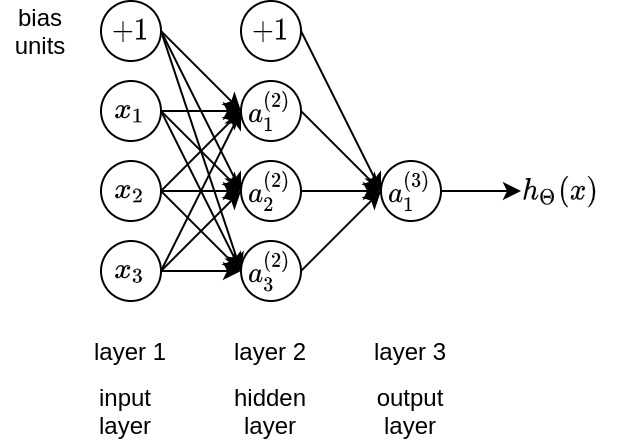
\includegraphics[scale=0.4]{./images/neural_network.jpg}
\end{center}
\[a_i^{(j)} = \text{"activation" of unit i in layer j}\]
\[\Theta^{(j)} = \text{matrix of weights (edges) from layer j to j + 1}\]

\bigskip

\[a_1^{(2)} = g(\Theta_{10}^{(1)} x_0 + \Theta_{11}^{(1)} x_1 + \Theta_{12}^{(1)} x_2 + \Theta_{13}^{(1)} x_3)\]
\[a_2^{(2)} = g(\Theta_{20}^{(1)} x_0 + \Theta_{21}^{(1)} x_1 + \Theta_{22}^{(1)} x_2 + \Theta_{23}^{(1)} x_3)\]
\[a_3^{(2)} = g(\Theta_{30}^{(1)} x_0 + \Theta_{31}^{(1)} x_1 + \Theta_{32}^{(1)} x_2 + \Theta_{33}^{(1)} x_3)\]
\[h_{\Theta}(x) = a_1^{(3)} = g(\Theta_{10}^{(2)} a_0^{(2)} + \Theta_{11}^{(2)} a_1^{(2)} + \Theta_{12}^{(2)} a_2^{(2)} + \Theta_{13}^{(2)} a_3^{(2)})\]

\bigskip

\noindent If network has \(s_j\) units in layer \(j\), \(s_{j + 1}\) units in layer \(j + 1\), then \(\Theta_j\) will be of dimension \(s_{j + 1} \times (s_j + 1)\).

\subsection{Simple Applications}

\begin{center}
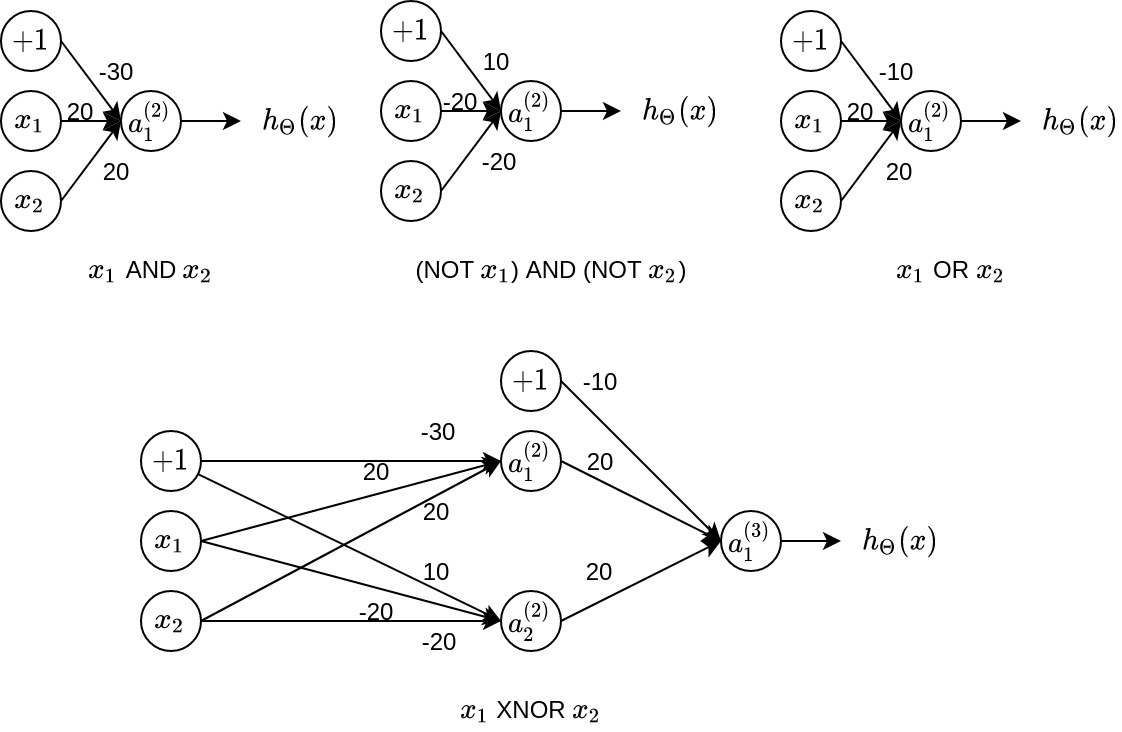
\includegraphics[scale=0.3]{./images/neural_network_simple_applications.jpg}
\end{center}

\subsection{Generalized Model}

\begin{center}
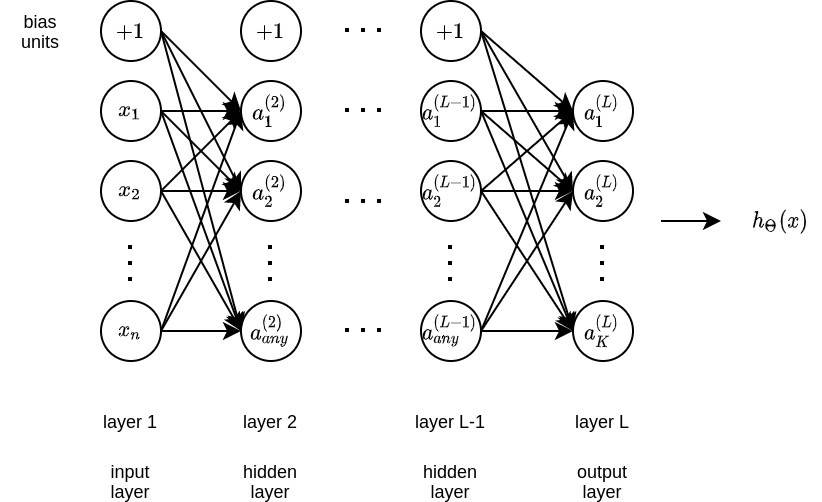
\includegraphics[scale=0.4]{./images/neural_network_generalized.jpg}
\end{center}

\noindent For a neural network that has:

\[L = \text{total number of layers in the network}\]
\[s_l = \text{number of units (not counting bias unit) in layer } l\]
\[K = \text{number of output units/classes}\]

\noindent assume \(a^{(1)} = x, a^{(L)} = h_\Theta(x)\), let:

\[z^{(l)} = \Theta^{(l - 1)} a^{(l - 1)}\]
\[a^{(l)} = g(z^{(l)})\]
\[h_\Theta(x) = a^{(L)} = g(z^{(L)})\]

\noindent Notice that bias units (\(a_0^{(l)} = 1\)) are considered as input only when calculating the next layer. They are not included in the output generated by previous layer.

\printindex

\end{document}